\documentclass[12pt, a4paper]{article}
\usepackage{amsmath, amssymb, mathrsfs}
\usepackage{graphicx}
\usepackage{url}
\usepackage{natbib}
\usepackage[margin=1in]{geometry}
\usepackage{braket}
\usepackage{bm}
\usepackage{tikz}
\usetikzlibrary{arrows.meta, decorations.pathmorphing, shapes.geometric, positioning}

\begin{document}

% Casimir Plates Diagram
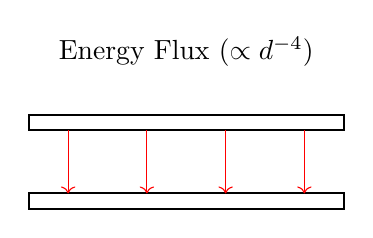
\begin{tikzpicture}
\draw[thick] (0,0) rectangle (4,0.2);
\draw[thick] (0,1) rectangle (4,1.2);
\foreach \x in {0.5,1.5,...,3.5} {
  \draw[->, red] (\x,1) -- (\x,0.2);
}
\node at (2,2) {Energy Flux (\(\propto d^{-4}\))};
\end{tikzpicture}
\bibliographystyle{plainnat}
\bibliography{references}

\end{document}
